%%%%%%%%%%%%%%%%%%%%%%%%%%%%%%%
% CHAPTER 4: EXPLORATORY STUDY
%%%%%%%%%%%%%%%%%%%%%%%%%%%%%%%
%% INTRODUCTION
%%%%%%%%%%%%%%%%%%%%%%%%%%%%%%%%%%%%%%%%%%%%%%%
%%%%%%%%%%%%%%%%%%%%%%%%%%%%%%%%%%%%%%%%%%%%%%%%
\section{Introduction}
\label{exp-study:introduction}
%%%%%%%%%%%%%%%%%%%%%%%%%%%%%%%%%%%%%%%%%%%%%%%%
%%%%%%%%%%%%%%%%%%%%%%%%%%%%%%%%%%%%%%%%%%%%%%%%

%%%%%%%%%%%%%%%%%%%%%%%%%%%%%%%%%%%%%%%%%%%%%
% ABBREVIATIONS
% SP SIGNPOSTING
%%%%%%%%%%%%%%%%%%%%%%%%%%%%%%%%%%%%%%%%%%%%%
% SECTION TODOs
% * Fix section references to earlier chapters
% * THINK: can I structure relative to CF?
%%%%%%%%%%%%%%%%%%%%%%%%%%%%%%%%%%%%%%%%%%%%%
% CONTENT
% Add as driver QUESTION: do results hold across multiple tools?
% Tone down critcisms and frame as `open research questions'
%%%%%%%%%%%%%%%%%%%%%%%%%%%%%%%%%%%%%%%%%%%%%

%%%%%%%%%%%%%%%%%%%%%%%%%%%%%%%%%%%%%%%%%%%%%%%%%%
% CHAPTER INTRO
% * bang bang bang intro, straight into aims - MUST BE PERSUASIVE
% * Need to relate Chapter aims to Thesis aims
%%%%%%%%%%%%%%%%%%%%%%%%%%%%%%%%%%%%%%%%%%%%%%%%%%
% \footnote{This draft of Chapter 4 Exploratory cross-tool study was printed \today}
% Twenty-five participants were interviewed over the period from from Autumn 2000 to Summer 2002.
% This \textit{cross-tool} perspective goes beyond previous work by allowing the construction of a cross-tool profile of user behaviour.  
% \textbf{Chapter~\ref{chapter:exploratory_study}}
% It was envisaged that such cross-tool data would provide guidance for the design of PIM-tool integration mechanisms.
This chapter reports an exploratory study of everyday Personal Information Management (PIM) practices.  A key objective of this study was to develop a holistic understanding of participants' PIM behaviour by collecting data across three PIM-tools: files, email and bookmarks. The study's cross-tool scope differentiates it from most previous studies in the area which have focused on specific PIM-tools (see \textbf{Section~\ref{review:pim-empirical-review}}).
% In contrast, previous studies have focused on \textit{specific} PIM-tools such as email (e.g.~\citep{Whittaker-email:96}, 
\textbf{Figure~\ref{fig:exp-study:intra_versus_cross_tool}} compares previous \textit{tool-specific} studies, with the the \textit{cross-tool} approach employed here.
% These two perspectives, tool-specific and cross-tool, are compared in  The tool-specific approach as employed in previous studies allows the \textit{within-tool/between-users} characterization of PIM practices within particular tool.  In contrast the cross-tool approach employed here enabled the comparison of practices between tools.    % This cross-tool nature of the study reported here allowed the comparison of behaviour between different PIM-tools. 
%%%%%%%%%%%%%%%%%%%%%%%%%%%%%%%%%%%%%%%%%%%%%%%%%%%%%%%%%%%%%%%%%%%%%%%%%%
% Describe the two cross-tool analysis approaches
% (1) comparison of generalized/aggregate data AND (2) within-user profile
%%%%%%%%%%%%%%%%%%%%%%%%%%%%%%%%%%%%%%%%%%%%%%%%%%%%%%%%%%%%%%%%%%%%%%%%%%
% In this study, cross-tool analysis was carried out from two perspectives: (1) comparing generalized behaviour, aggregated across all participants, and (2) comparing practices between tools for specific users. More detail is provided on each perspective below.
% The first perspective involved the comparison of \textit{generalized} behaviour between the three PIM-tools. To cover all aspects of PIM, interviews were structured to cover Barreau's four PIM sub-activities in each collection.  This analytical perspective is equivalent to carrying out three tool-specific studies in parallel. In the chapter, a novel technique is proposed to compare the tools in terms of the \textit{organizational dimensions} used to name folders in each PIM-tool.
%%%%%%%%%%%%%%%%%%%%%%%%%%%%%%%
% between-tools/within-user
%%%%%%%%%%%%%%%%%%%%%%%%%%%%%%%
% The second perspective involved \textit{between-tools/within-user} analysis to compare PIM practices across all three tools for each participant. A novel technique is presented to construct a \textit{cross-tool profile} for each participant in terms of the extent to which they organized multiple types of information.  This contrasts with previous strategy profiling which has only been carried out in the context of specific tools.
% A second technique is proposed to assess the similarity of folder structures in different PIM-tools based on the level of \textit{folder overlap}.
% Finally the cross-tool profiles were categorized to develop a classification of cross-tool PIM practices across all participants.
% Three new analytical techniques were employed in the study: analysis of \textit{organizational dimensions}, \textit{cross-tool profiling} and analysis of \textit{folder overlap}.

% %%%%%%%%%%%%%%%%%%%%%%%%%%%%%
% FIGURE - Intra-tool/Cross-tool Comparison
% %%%%%%%%%%%%%%%%%%%%%%%%%%%%%
\begin{figure}[hbtp]
	\begin{center}
		\leavevmode
		% height=2in, width=.9 \textwidth
		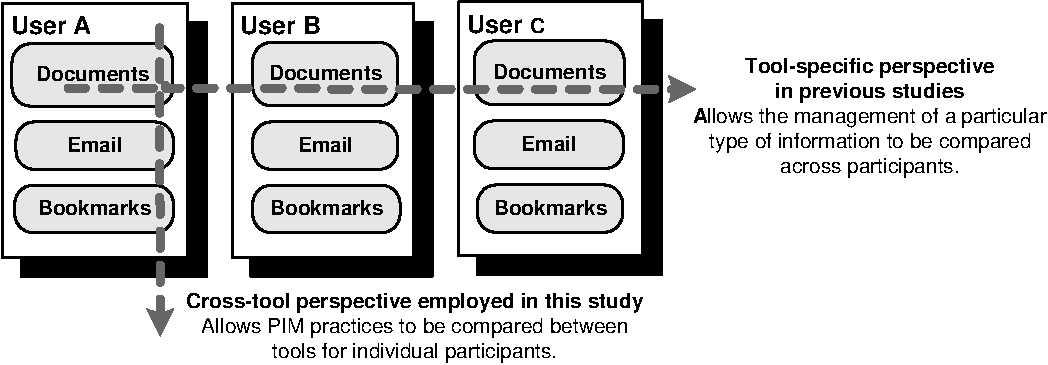
\includegraphics[height=4cm]{pictures/exp-study/exp-study-intracrosscomparison.pdf}
		\caption{Comparing the cross-tool and tool-specific study perspectives.} 	% The two analytical perspectives used in PIM studies: (1) tool-specific (within-tool/between-users); and (2) cross-tool (between-tools/within-user).}
		\label{fig:exp-study:intra_versus_cross_tool}
	\end{center}
\end{figure}

%%%%%%%%%%%%%%%%%%
% LINK FORWARDS
%%%%%%%%%%%%%%%%%%
% This section details the chapter's contributions towards the overall thesis.
% This chapter acts as an empirical foundation for the rest of the thesis.
The findings in this chapter, combined with the insights reported in \textbf{Chapter~\ref{chapter:review}}, provide an empirical grounding for the design work in \textbf{Chapter~\ref{chapter:design}}.
% Lessons learned in carrying out the exploratory study also help shape the methodology employed in the subsequent empirical work reported in \textbf{Chapters~\ref{chapter:design}} and \textbf{\ref{chapter:main-study}}.
% The study also contributed to the development of the cross-tool analytical framework outlined in \textbf{Chapter~\ref{chapter:discussion}}.
The work presented in this chapter has been reported in a number of publications ~\citep{rpb:01b,rpb:02c,rpb:03a,rpb:04a}.


%%%%%%%%%%%%%%%%%%%%%%%%%%%%%
% LINK TO REST OF SECTION
%%%%%%%%%%%%%%%%%%%%%%%%%%%%%
% The rest of this section is structured as follows. Firstly \textbf{Section~\ref{exp-study:objectives}} presents the study's objectives. Then \textbf{Section~\ref{exp-study:study-scope}} reports decisions made to limit the study's scope of inquiry. \textbf{Section~\ref{exp-study:contributions}} discusses the chapter's contributions towards the overall thesis.  

%%%%%%%%%%%%%%%%%
%%%%%%%%%%%%%%%%%
%%%%%%%%%%%%%%%%%
%%%%%%%%%%%%%%%%%

%%%%%%%%%%%%%%%%%%%%%%%%
\subsection{Objectives}
\label{exp-study:objectives}
%%%%%%%%%%%%%%%%%%%%%%%%

The study objectives were as follows:
\begin{enumerate}

%%%%%%%%%%%%%%%%%%%%%%%%%%%%%%%%%%%%
% OBJECTIVE 1: Cross-tool Knowledge
%%%%%%%%%%%%%%%%%%%%%%%%%%%%%%%%%%%%%%%%%%%%%%%%%%%%%%%%%%%%%%%%%%%%%%%%%%%%%%%%%%%%%%%%%%%%%%%%%%%%%%%%%%%%
% FROM CHI04: Although many innovative designs have been proposed, WE see a mismatch between the tool-specific studies that have provided observations about users� activities and problems � and the substantial design effort directed at cross-tool integration. There is a need for cross-tool empirical data to provide a foundation for such cross-tool design.
% FROM CHI04: Our study aimed to build on previous research in two ways: 1.	
%%%%%%%%%%%%%%%%%%%%%%%%%%%%%%%%%%%%%%%%%%%%%%%%%%%%%%%%%%%%%%%%%%%%%%%%%%%%%%%%%%%%%%%%%%%%%%%%%%%%%%%%%%%%
% NB: consider exceptions, eg CM, TKM
%%%%%%%%%%%%%%%%%%%%%%%%%%%%%%%%%%%%%%%%%%%%%%%%%%%%%%%%%%%%%%%%%%%%%%%%%%%%%%%%%%%%%%%%%%%%%%%%%%%%%%%%%%%%
%% To provide a cross-tool empirical foundation for the thesis by investigating participants' PIM practices across three collections of information: files, email, and bookmarks. 
% and to develop a rich picture of PIM behaviour across a range of tools.
% To provide a more effective foundation for cross-tool design, WE profiled participants' practices in  It was envisaged that cross-tool data would be useful in establishing an empirically-grounded foundation 
%% In particular a key motivation behind this research programme was an interest in exploring the potential to improve integration between PIM tools. \textit{Thus the above high-level objectives should be considered in the context of this interest.} 
%%%%%%%%%%%%%%%%%%%%%%%%%%%%%%%%%%%%%%%%%%%%%%%%%%%%%%%%%%%%%%%%%%%%%%%%%%%%%%%%%%%%%%%%%%%%%%%%%%%%%%%%%%%%
\item	\textit{To compare how users manage different types of personal information} -- \textbf{Section~\ref{review:pim-technological-review}} identified a mismatch between the \textit{tool-specific} empirical studies that have provided observations about PIM behaviour and problems, and the substantial \textit{cross-tool} design effort directed at improving integration between PIM tools.  Furthermore, it was argued that much of this design work has been based on designer intuition rather than empirical data.  A case was made for more cross-tool empirical data to provide an effective empirical foundation for the design of integration mechanisms. % surveyed the substantial design effort that has been directed at improving integration between PIM tools. 

The primary aim of this study was to take steps towards addressing this research gap.  To achieve this, participants' PIM practices were profiled across three commonly managed collections of personal information: (1) document files, (2) email messages and (3) web bookmarks -- managed within the file system, email tool and web browser respectively. 

%%%%%%%%%%%%%%%%%%%%%
% OBJECTIVE 2: Design foundation
%%%%%%%%%%%%%%%%%%%%%
%   By developing understanding of PIM from a cross-tool perspective, it was envisaged that the study would provide requirements and ideas for subsequent design work.
\item \textit{To provide motivation and requirements for subsequent design} -- An orienting commitment in this research was to design and evaluate a novel PIM-integration mechanism.  It was hoped that the study findings would guide subsequent design work. % within this programme of research.

%%%%%%%%%%%%%%%%%%%%%%%%%%%%%%%%%%%%
% OBJECTIVE 2: General knowledge including tool-specific knowledge
%%%%%%%%%%%%%%%%%%%%%%%%%%%%%%%%%%%%
%%%%%%%%%%
% NOTES
% * need base understanding in specific tools to build up cross-tool understanding
% * change to familiarise himself?
% * Mention fact that do not discuss individual PIM-tools in depth, for this see previous studies.
%%%%%%%%%%%%
\item	\textit{To provide background on PIM} -- \textbf{Chapter~\ref{chapter:review}} highlights the lack of a systematic knowledge base of empirical data relating to PIM.   In addition to building up a \textit{cross-tool} understanding of PIM, the study was seen as an opportunity for the author to ``get his hands dirty'' and familiarise himself with a range of PIM-related issues, e.g. those relating to specific PIM-tools.
% develop a first-hand appreciation of user needs.
% author hoped to ,   In general, the study was seen as an opportunity for the author 

%%%%%%%%%%%%%%%%%
% OBJECTIVE 3: Research focus
%%%%%%%%%%%%%%%%%
\item \textit{To confirm a research focus} -- Since PIM is a complex activity and offers a wide range of compelling research problems (see~\textbf{Chapter~\ref{chapter:introduction}}), the author perceived a strong need to focus his research efforts.  % NB: fix section reference
The exploratory study was intended to help identify an interesting, worthwhile and achievable research problem. % i.e. justify research focus

\end{enumerate}

%%%%%%%%%%%%%%%%%
%%%%%%%%%%%%%%%%%
%%%%%%%%%%%%%%%%%
%%%%%%%%%%%%%%%%%

%%%%%%%%%%%%%%%%%%%%%%%%%%%%%%%
\subsection{Study scope}
\label{exp-study:study-scope}
% \textbf{Section~\ref{exp-study:studyscope}} 
%%%%%%%%%%%%%%%%%%%%%%%%%%%%%%%
% This section details the decisions taken by the author to limit the study scope.
% \textbf{Chapter~\ref{chapter:bg}} outlines the complex nature of PIM as an idiosyncratic, ongoing activity made up of four key sub-activities (acquisition, organization, maintenance and retrieval). The challenges inherent in investigating such a long-term, multifaceted activity, were compounded by the intention to investigate PIM across a range of tools. 
% One consequence of widening the scope of enquiry to encompass multiple tools is that the complexity of the HCI phenomena being investigated is increased. 
% Faced with the potential of such analytical complexity, the following constraints were applied to limit the study's scope:
%%
%% \footnote{\textit{NOTE TO READERS OF DRAFT: \textbf{Figure~\ref{fig:chapter1_pim_model}} is included at the end of this section to illustrate the analytical framework that I use for talking about PIM (based on that of~\citep{barreau:95}). Note that in the final version this conceptual grounding will be located in the introductory chapter}}.
The primary aim of the study, to investigate a complex activity such as PIM from a holistic, \textit{cross-tool} perspective, was clearly an ambitious one.  In order to offset the potential analytical complexity, the scope of the study was constrained in the following ways:

\begin{enumerate}

%%%%%%%%%%%%%%%%	
% SCOPE LIMIT 1
%%%%%%%%%%%%%%%%
% : the primary desktop workspace
\item \textit{Focus on PIM practice within the context of a single personal computer} -- The domain of interest was limited to the computer where each participant performed the majority of their computer-based activity at their place of work. Thus the extra complexity of considering PIM on multiple computers and mobile devices was avoided.

%%%%%%%%%%%%%%%%
% SCOPE LIMIT 2
%%%%%%%%%%%%%%%%
% digital and physical tools to manage personal information 
% Fix figure reference ~\ref{fig:chapter1_workspace}}). 
\item \textit{Focus on three PIM-tools} -- Even within the context of one computer, users often employ a wide and varying range of PIM-tools (see \textbf{Figure~\ref{fig:chapter2_pie}}). 
Due to time constraints, it was decided to focus the study on three commonly-used PIM-tools: files, email and web bookmarks.  A further focus was taken on the management of \textit{personal document files} within the file system, as described in \textbf{Section~\ref{exp-study:interview-process}}.
% Although the core of the study focused on these three collections, enquiries were made regarding other PIM tools (e.g. address books and calendars) if time allowed.

%%%%%%%%%%%%%%%%
% SCOPE LIMIT 3
%%%%%%%%%%%%%%%%
\item \textit{Non-longitudinal study} -- As noted in \textbf{Chapter~\ref{chapter:review}}, PIM is an ongoing activity, and user behaviour may evolve over time~\citep{ob:97}.  However, due to time constraints, and likemost previous studies, this investigation was based on a one-off ``snapshot'' of behaviour\footnote{In the exploratory study, it was still possible to collect data relating to longitudinal issues (e.g. changes in strategy) in the form of historical reports offered by participants.  \textbf{Chapter~\ref{chapter:main-study}} reports a follow-up longitudinal study carried out by the author that captured data over time.}.

%%%%%%%%%%%%%%%%
% SCOPE LIMIT 4
%%%%%%%%%%%%%%%%
 % For example the members of a team may each store personal information in a shared email account or within a sub-folder on a network drive.
%% THINK: this small print can be encapsulated in definition in Background chapter
%% Such as: what are the extra issues concerned with collaborative information management
% cite Collaborative Information Management issues (e.g. Berlin et al. 1993)
\item \textit{Focus on personal rather than shared information} -- As noted in \textbf{Chapter~\ref{chapter:bg}}, a user may store personal information within a group information space, such as a network drive shared with colleagues. To avoid taking into account the issues related to collaboration, this study focused on information that was not shared with other users.

\end{enumerate}

%%%%%%%%%%%%%%%%%
%%%%%%%%%%%%%%%%%
%%%%%%%%%%%%%%%%%
%%%%%%%%%%%%%%%%%


	





%%%%%%%%%%%%%%%%%%%%%%%%%%%%%%%%%%%%%%%%%%%%%%
\subsection{Contributions}
\label{exp-study:contributions}
% \textbf{Section~\ref{exp-study:contributions}}
%%%%%%%%%%%%%%%%%%%%%%%%%%%%%%%%%%%%%%%%%%%%%%

The following methodological and substantive contributions are offered in the chapter:
%% NB: for all of these, must relate to SO WHAT?
% The first set of substantive contributions resulted from the \textit{within-tool/between-users} analysis. ALSO CONSIDER: SO WHAT!!
% (perspective 1 in~\textbf{Figure~\ref{fig:chapter3_intra_versus_cross_tool}}):
\begin{enumerate}

%%%%%%%%%%%%%%%%%%%%%%%%%%%%%%%%%%%%%%%%%%%%%%%
% CONTRIB B: COMPARISON OF STRATS IN TOOLS
%%%%%%%%%%%%%%%%%%%%%%%%%%%%%%%%%%%%%%%%%%%%%%%
% by capturing data across multiple tools for each participant
% The second set of substantive contributions result from the \textit{between-tools/within-user} analysis:
% ADD: SO WHAT: Implications are discussed in XYZ
% The study's primary contribution is in terms of \textit{improved cross-tool understanding of PIM}. A high-level comparison of management strategies is presented in \textbf{Section~\ref{exp-study:Results-comparison}} to contrast behaviour between the file, email, and bookmark collections across all the participants.
% This initial cross-tool comparison is based on the generalized views of user behaviour developed in the \textit{within-tool/between-user} analysis.
% The cross-tool analysis is used to derive a set of design implications for improving tool integration.
\item \textit{A comparison of PIM behaviour between the three PIM-tools} -- \textbf{Section~\ref{exp-study:Results-comparison}} presents a high-level comparison between files, email and bookmarks in terms of four PIM sub-activities (acquisition, organization, maintenance and retrieval).  This data emphasises how the nature of PIM varies between different PIM-tools.


%%%%%%%%%%%%%%%%%%%%%%%%%%%%%%%%%%%%%%%%%%%%%%%%%%%%%%%%%%%%%%
% CONTRIB E: NEW METHOD OF C/T PROFILING AND APPLICATION
%%%%%%%%%%%%%%%%%%%%%%%%%%%%%%%%%%%%%%%%%%%%%%%%%%%%%%%%%%%%%%
% A method of performing the cross-tool profiling of users. The method is applied here to illustrate the variation in terms of extent of filing across tools for many participants. Evidence of multiple strategies at a cross-tool level for many people.
\item \textit{A comparison of organizing strategies between the three PIM tools} -- A focus is taken on the organizing sub-activity in \textbf{Section~\ref{exp-study:Results-org-strategies}}, where it is observed that many individuals employ a rich variety of organizing strategies \textit{both within and across PIM tools}.  Previous classifications of organizing behaviour are criticised for not reflecting this behaviour, and new classifications are offered for tool-specific and cross-tool contexts.  
% \textbf{Section~\ref{exp-study:discussion:multiple-strategies}} presents a model to describe the observations of multiple strategies in tool-specific and cross-tool contexts.
% The second methodological contribution is that of \textit{cross-tool profiling}. 
% A classification of PIM behaviour is presented to indicate the extent of user's organizing across multiple tools.

%%%%%%%%%%%%%%%%%%%%%%%%%%%%%%%%%%%%%%%%%%%%%%%%%%%%%%%%%%%%%%
% CONTRIB C: NEW METHOD OF ORG DIM ANALYSIS AND APPLICATION
%%%%%%%%%%%%%%%%%%%%%%%%%%%%%%%%%%%%%%%%%%%%%%%%%%%%%%%%%%%%%%
% \item An new method and application of analysis of the organizational dimensions used to name folders in each tool. This is used to criticise PIM-integration based on one organizational dimension.
% (the types of concept, e.g. people, projects, places on which folder names are
\item \textit{The development and application of a novel technique for comparing the organizational dimensions on which folders are based in each PIM-tool} -- Organizational dimensions are defined as the types of concept on which folder names are based (e.g. project or interest).  The method employed is described in \textbf{Section~\ref{exp-study:folder-analysis-orgdim}}.  The results in \textbf{Section~\ref{exp-study:Results-org-dims}} highlight the range of dimensions employed by users to name folders in the three PIM-tools. A number of previous PIM-integration systems are criticised for focusing on one type of organizational dimension.

%%%%%%%%%%%%%%%%%%%%%%%%%%%%%%%%%%%%%%%%%%%%%%%%%%%%%%%%%%%%%%
% CONTRIB D: NEW METHOD OF F/O ANALYSIS AND APPLICATION
%%%%%%%%%%%%%%%%%%%%%%%%%%%%%%%%%%%%%%%%%%%%%%%%%%%%%%%%%%%%%%
\item \textit{The development and application of a novel technique for assessing the similarity of a user's file, email and bookmark folder structures in terms of overlapping folders} -- The method is documented in \textbf{Section~\ref{exp-study:analysis-folder-overlap}}, and results are presented in \textbf{Section~\ref{exp-study:Results-folder-overlap}}. Significant folder overlap is observed for most study participants, particularly between their file and email collections.  These results provide a key design motivation for the WorkspaceMirror tool presented in \textbf{Chapter~\ref{chapter:design}}.
% Folder overlap is proposed as a means of assessing the similarity of two structured collections of personal information.
% A new method and application of analysis of the extent of folder overlap between the tools

%%%%%%%%%%%%%%%%%%%%%%%%%%%%%%%%%%
%  SUBSTANTIVE 6: General implications for design
%%%%%%%%%%%%%%%%%%%%%%%%%%%%%%%%%%
\item \textit{Implications for the design of PIM-integration mechanisms} -- \textbf{Section~\ref{exp-study:comparison-problems}} highlights a range of cross-tool problems highlighting the potential of improving integration between PIM-tools.  \textbf{Section~\ref{exp-study:conclusion}} presents a number of design implications for improving tool integration, based on the findings in the chapter. 
% The cross-tool findings are used to argue for possible routes for integrating between tools, see \textbf{Section~\ref{exp-study:conclusion}}.  Synergies and differences between tools that may be useful in guiding the design of tool integration. % The cross-tool findings are used to argue for possible routes for integrating between tools, see \textbf{Section~\ref{exp-study:conclusion}}.  Synergies and differences between tools that may be useful in guiding the design of tool integration. 
% It is argued that such cross-tool understanding may identify synergies and dissimilarities between tools that can indicate appropriate routes for integrating them.

%%%%%%%%%%%%%%%%%%%%%%%%%%%%%%%%%%%%%%%%%%%%%%%%%%
% SUBSTANTIVE 1: Increased understanding in specific tools: WTBU
% CONTRIB A: T/S -> NEW T/S STRATS
%%%%%%%%%%%%%%%%%%%%%%%%%%%%%%%%%%%%%%%%%%%%%%%%%%
% \item Enhanced understanding of PIM within the tool-specific contexts of files, email and bookmarks.
%  New classifications of organizing strategies were offered in each context.  Evidence of multiple strategies in tool-specific contexts.
% Previous classifications of email and bookmark management strategies are criticised for not reflecting this behaviour. A new classification of file management behaviour is proposed. 
% MOVE TO CONTRIBUTIONS This analytical perspective is equivalent to the approach pursued in previous tool-specific studies, and was intended to confirm and build on previous findings.
% ADD: SO WHAT: Implications are discussed in XYZ
\item \textit{Improved understanding of PIM behaviour in specific tools} -- Although not the primary aim of the study, several incremental tool-specific contributions are provided. In particular, \textbf{Section~\ref{exp-study:Results-org-strategies}} offers new classifications of organizing behaviour in files, email and bookmarks.  \textbf{Section~\ref{exp-study:Results-org-dims}} characterizes the types of folders developed in each tool.

\end{enumerate}
%The three methodological contributions consisted of the three analytical techniques developed by the author:


%%%%%%%%%%%%%%%%%
%%%%%%%%%%%%%%%%%
%%%%%%%%%%%%%%%%%
%%%%%%%%%%%%%%%%%


%%%%%%%%%%%%%%%%%%%%%%%%%%%%%%%
\subsection{Structure of the Chapter}
\label{exp-study:structure}
% \textbf{Section~\ref{exp-study:studyscope}} 
%%%%%%%%%%%%%%%%%%%%%%%%%%%%%%%

%%%%%%%%%%%%%%%%%
% SIGNPOSTING
%%%%%%%%%%%%%%%%%
The rest of \textbf{Chapter~\ref{chapter:exploratory_study}} is structured as follows.
\textbf{Section~\ref{exp-study:method}} reports the study method, including choice of participants, data collection, and data analysis.  \textbf{Section~\ref{exp-study:results-overview}} provides an overview of the study results which are presented over \textbf{Sections~\ref{exp-study:Results-comparison}} to \textbf{\ref{exp-study:comparison-problems}}.
% , their limitations, and contributions towards the overall thesis.
% explores the implications following from the results of the study.
Finally, \textbf{Section~\ref{exp-study:conclusion}} discusses the main findings from the chapter.

%%%%%%%%%%%%%
% END INTRO
%%%%%%%%%%%%%

%